
\chapter{Motivating Examples} % Main chapter title

\label{Chapter7} % For referencing the chapter elsewhere, use \ref{Chapter1} 

\lhead{Chapter 7. \emph{Motivating Examples}} % This is for the header on each page - perhaps a shortened title

\section{Example 1: Resource Allocation for a mixed criticality workload}

\subsection{Intro}
Recent work has examined automated design space exploration to map applications onto heterogeneous multicore platforms \cite{bolchini2013reliability,huang2014framework}. Figure \ref{f:motiv_ex} shows an example task graph for a set of critical tasks as well as a pool of unrelated non-critical tasks. The platform in question consists of one fault tolerant core and 4 plain cores with fingerprinting units. The benefits of ODR should be apparent right from time 0 since four non critical tasks are able to execute concurrently. As for DCC, consider what happens at time 80. There is only one non-critical task (NCT) remaining once critcal task (CT) 3 is complete. Meanwhile, CT4 cannot begin until time 100 when CT-2 is also completed. Core 3 remains busy until time 90 on NCT-d. By allowing C2 and C3 to execute CT4, C1 is freed up to begin execution of NCTf immediately.

\begin{figure}[ht]
\centering
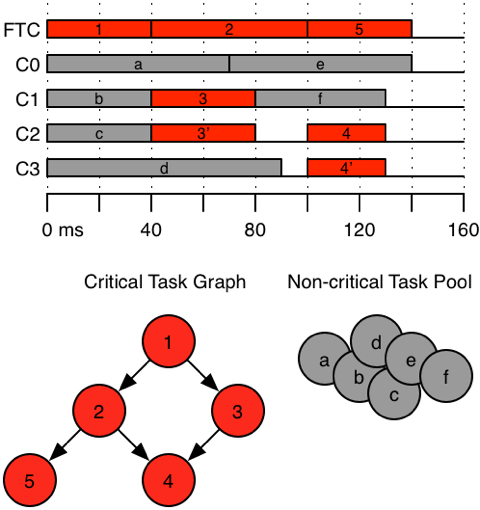
\includegraphics[scale=0.8]{Figures/motiv_ex.png}
\caption[Resource Allocation for a mixed criticality workload] {\emph{Resource Allocation for a mixed criticality workload}: A set of critical tasks with dependencies and non-critical tasks are mapped onto the platform. ODR and DCC allow a much higher non-critical workload to be executed.}
\label{f:motiv_ex}
\end{figure}

\subsection{Result}
We execute this schedule on a platform with five Nios cores, four of which have fingerprinting units. The fifth is assumed to be the FTC. The cores are synchronized to a global time and are each responsible for their own static schedule. Software services handling the recovery from errors and calculation of alternative schedules in the case of faults are beyond the scope of the present work. The system is set up as follows:

\begin{itemize}
\item The monitor completes execution of task 1.
\item In between task 1 and 2, the monitor initializes the comparator (setting the directory for task 3 as well as the core assignment table.
\item After task 3 has completed, an interrupt is sent from the comparator to the fault tolerant core to notify it that task 3 has completed successfully.
\item After task 2 has completed, the fault tolerant core reprograms the directory and core assignment table for task 4 to execute
\item Global time is maintained using loosely synchronized local timers. Timekeeping of all cores is not disrupted. Although the tasks span 4-7 clock ticks, it is not necessary to disable the interrupts since they do not corrupt the fingerprinting process.
\item \emph{note:} It is not strictly necessary for the different critical tasks to have different FIDs. This would save the FTC from having to reprogram the directory as well.
\item \emph{note:} We have stripped the tasks of all message passing. The system is only implemented in enough detail to demonstrate the correct functionality of the novel hardware and the resulting possibilities for higher level scheduling.
\end{itemize}

\section{Example 2: Fingerprinting a Simulink generated control loop}
\subsection{Intro}

We firmly hold that the new design must be easily integrate with existing tools and require only minor cosmetic changes to the standard outputs from those tools. Model based design is fundamental to automotive software engineering. An increasing proportion of the millions of lines of code that are currently used to run modern cars are computer generated. Furthermore, whether soft core or hard core, ISAs are well established and compiler tool chains are mature and stable. This second example demonstrates how fingerprinting can be used to monitor redundant executions of Simulink generated control code integrated into a simple RTOS template and compiled with \emph{gcc}.

Simulink Coder was used to extract transmission control logic from an example of an automotive drive train model \cite{sim_trans}. It would defeat the purpose and convenience of Coder to be forced to comb through and restructure the code to obey some style that is not natively supported. There are two things to note about the style of code: one that supports ease of fingerprinting and one that requires more attention. Firstly, the algorithm is a discrete FSM that will deterministically produce the same outputs given identical inputs. The tasks will match at the instruction level. The areas requiring more attention is the handling of global variables. Since the code will make hardwired references to global variables (i.e. the compiler will insert the absolute addresses into load and store instructions or calculate their position based on a global pointer register) it is necessary to ensure that separate duplicate copies are made for each core and that neither core is able to corrupt the original copy until fingerprinting is completed and the tasks are known to have been successful. 

Memory protection strategies is currently outside the scope of this work but the technology for implementing them is obviously well established. We assume that mechanisms are in place such that it is not physically possible for either plain core to write to the original data once a copy has been made. The final writeback must be done by reliable DMA initiated by a fault tolerant core (A core might be required to move the data out of the scratchpad to make room for another task or to provide a reference copy of data for rollback/reexecution purposes).

Once the global variables are copied into the scratchpads of the plain cores, memory translation is enabled to reroute references to global references away from main memory to the scratchpad. A full power MMU and OS virtualization services are not required. It is sufficient to ensure using linker options that the global variables are located in a contiguous block of data page aligned in accordance with the tag size of the uTLB. Meanwhile, the task stack must also be fit into the scratchpad and is accessed using its local physical address. As a further precaution, the global pointer register on each core are changed to match the GP register of whichever core the critical tasks were compiled for in case the compiler inserts GP relative address calculations. The context switch assembly code located in the BSP is then updated to include saving, resetting, and restoring the global pointer register so that any local interrupt handling code is not corrupted by a modified global pointer register should an interrupt occur during the critical task.



